\documentclass[12pt]{report}
\usepackage[utf8]{inputenc}
\usepackage[english, russian]{babel}
\usepackage{listings}
\usepackage{graphicx}
\usepackage{float}
\graphicspath{{imgs/}}
\usepackage{amsmath,amsfonts,amssymb,amsthm,mathtools} 
\usepackage{pgfplots}
\usepackage{filecontents}
\usepackage{indentfirst}
\usepackage{eucal}
\usepackage{enumitem}
\frenchspacing

\usepackage{indentfirst} % Красная строка

\usetikzlibrary{datavisualization}
\usetikzlibrary{datavisualization.formats.functions}

\usepackage{amsmath}
\usepackage{fixltx2e}
\usepackage{caption}


\definecolor{bluekeywords}{rgb}{0,0,1}
\definecolor{greencomments}{rgb}{0,0.5,0}
\definecolor{redstrings}{rgb}{0.64,0.08,0.08}
\definecolor{xmlcomments}{rgb}{0.5,0.5,0.5}
\definecolor{types}{rgb}{0.17,0.57,0.68}

\usepackage{listings}
\lstset{language=[Sharp]C,
	captionpos=t,
	numbers=left, %Nummerierung
	numberstyle=\small, % kleine Zeilennummern
	frame=single, % Oberhalb und unterhalb des Listings ist eine Linie
	stepnumber=1,                   
	numbersep=5pt,                
	showspaces=false,
	tabsize=2,
	showtabs=false,
	breaklines=true,
	showstringspaces=false,
	breakatwhitespace=true,
	escapeinside={(*@}{@*)},
	commentstyle=\color{greencomments},
	morekeywords={partial, var, value, get, set},
	keywordstyle=\color{bluekeywords},
	stringstyle=\color{redstrings},
	basicstyle=\ttfamily\small,
}

\usepackage[left=2cm,right=2cm, top=2cm,bottom=2cm,bindingoffset=0cm]{geometry}
% Для измененных титулов глав:
\usepackage{titlesec, blindtext, color} % подключаем нужные пакеты
\definecolor{gray75}{gray}{0.75} % определяем цвет
\newcommand{\hsp}{\hspace{20pt}} % длина линии в 20pt
% titleformat определяет стиль
\titleformat{\chapter}[hang]{\Huge\bfseries}{\thechapter\hsp\textcolor{gray75}{|}\hsp}{0pt}{\Huge\bfseries}

\usepackage{array}
\newcommand{\head}[2]{\multicolumn{1}{>{\centering\arraybackslash}p{#1}}{#2}}

% plot
\usepackage{pgfplots}
\usepackage{filecontents}
\usetikzlibrary{datavisualization}
\usetikzlibrary{datavisualization.formats.functions}

\begin{document}
%\def\chaptername{} % убирает "Глава"
\thispagestyle{empty}
\begin{titlepage}
	\noindent \begin{minipage}{0.15\textwidth}
		
\includegraphics[width=\linewidth]{b_logo}
	\end{minipage}
	\noindent\begin{minipage}{0.9\textwidth}\centering
		\textbf{Министерство науки и высшего образования Российской Федерации}\\
		\textbf{Федеральное государственное бюджетное образовательное учреждение высшего образования}\\
		\textbf{~~~«Московский государственный технический университет имени Н.Э.~Баумана}\\
		\textbf{(национальный исследовательский университет)»}\\
		\textbf{(МГТУ им. Н.Э.~Баумана)}
	\end{minipage}
	
	\noindent\rule{18cm}{3pt}
	\newline\newline
	\noindent ФАКУЛЬТЕТ $\underline{\text{«Информатика и системы управления»}}$ \newline\newline
	\noindent КАФЕДРА $\underline{\text{«Программное обеспечение ЭВМ и информационные технологии»}}$\newline\newline\newline\newline\newline\newline\newline\newline\newline\newline\newline
	
	
	\begin{center}
		\noindent\begin{minipage}{1.3\textwidth}\centering
			\Large\textbf{  Отчет по лабораторной работе №4}\newline
			\textbf{по дисциплине \newline "Функциональное и логическое программирование"}\newline\newline
		\end{minipage}
	\end{center}
	
	\noindent\textbf{Тема} $\underline{\text{Использование управляющих структур, работа со списками}}$\newline\newline
	\noindent\textbf{Студент} $\underline{\text{Малышев И. А.}}$\newline\newline
	\noindent\textbf{Группа} $\underline{\text{ИУ7-61Б}}$\newline\newline
	\noindent\textbf{Оценка (баллы)} $\underline{\text{~~~~~~~~~~~~~~~~~~~~~~~~~~~}}$\newline\newline
	\noindent\textbf{Преподаватель: } $\underline{\text{Толпинская Н. Б.}}$\newline\newline\newline
	
	\begin{center}
		\vfill
		Москва~---~\the\year
		~г.
	\end{center}
\end{titlepage}


\setcounter{page}{2}
\chapter*{Теоретические вопросы}

\section*{1. Синтаксическая форма и хранение программы в памяти}

В Lisp формы представления программы и обрабатываемых ею данных одинаковы – они представлены в виде S-выражений. Программы могут обрабатывать и преобразовывать другие программы или сами себя. В памяти программа представляется в виде бинарных узлов, так как она состоит из S-выражений.\newline


\section*{2. Трактовка элементов списка}

Если отсутствует блокировка вычислений, то первый элемент списка трактуется как имя функции, а остальные элементы – как аргументы функции. На рисунке 1 представлена схема работы функции \textbf{eval}.

\begin{figure}[H]
	\begin{center}
		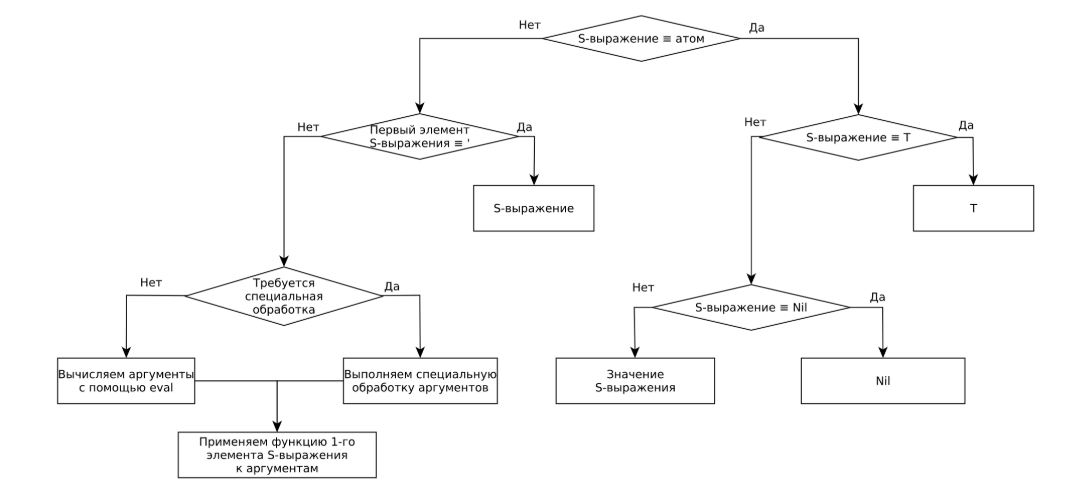
\includegraphics[scale=0.5]{imgs/eval.png}
	\end{center}
	\caption{Схема работы функции \textbf{eval}.}
	\label{img:eval}
\end{figure}

\section*{3. Порядок реализации программы}

Работа программы циклична: сначала программа ожидает ввода S-выражения, затем передает полученное S-выражение интерпретатору – функции eval, а в конце, после отработки функции eval, выводит последний полученный результат.\newline


\section*{4. Способы определения функции}

Определение функций пользователя в Lisp-е возможно двумя способами:
\begin{itemize}
	\item с использованием Лямбда-нотаци (функции без имени): (lambda (<аргументы>) (<тело>));
	\item с использованием макро определения DEFUN: (defun <имя> (<аргументы>) (<тело>)).
\end{itemize}



""\newline
\chapter*{Практические задания}

\subsection*{1. Чем принципиально отличаются функции cons, list, append?}

Пусть:
\begin{lstlisting}[label=6xd, language=lisp]
 	(setf lest1 '(a b)) 
	(setf lst2 '(c d)).
\end{lstlisting}	
Каковы результаты вычисления следующих выражений?

(cons lstl lst2) -> ((A B) C D)

(list lst1 lst2) -> ((A B) (C D))

(append lst1 lst2) -> (A B C D)


\subsection*{2. Каковы результаты вычисления следующих выражений, и почему?}

(reverse ()) -> Nil

(last ()) -> Nil

(reverse '(a)) -> (A)

(last '(a)) -> (A)

(reverse '((a b c))) -> ((A B C))

(last '((a b c))) -> ((A B C))

\subsection*{3. Написать, по крайней мере, два варианта функции, которая возвращает последний элемент
	своего списка-аргумента.}

\begin{lstlisting}[label=6xd, caption=Решение задания №3, language=lisp]
	(defun last-elem (lst) 
		(if (cdr lst) 
			(last-elem (cdr lst)) 
			(car lst)
		)
	)
	
	(defun last-elem (lst) (car (reverse lst)))

\end{lstlisting}

\subsection*{4. Написать, по крайней мере, два варианта функции, которая возвращает свой список-аргумент без последнего элемента.}

\begin{lstlisting}[label=6xd, caption=Решение задания №4, language=lisp]
	(defun no-last-elem (lst) (reverse (cdr (reverse lst))))



	(defun no-last-elem-internal (lst acc)
		(if (cdr lst)
			(no-last-elem-internal (cdr lst) (append acc (cons (car lst) Nil)))
			acc
		)
	)
	
	(defun no-last-elem (lst) (no-last-elem-internal lst ()))
\end{lstlisting}

\subsection*{5. Написать простой вариант игры в кости, в котором бросаются две правильные кости. Если
	сумма выпавших очков равна 7 или 11 -- выигрыш, если выпало (1,1) или (6,6) --- игрок право
	снова бросить кости, во всех остальных случаях ход переходит ко второму игроку, но
	запоминается сумма выпавших очков. Если второй игрок не выигрывает абсолютно, то
	выигрывает тот игрок, у которого больше очков. Результат игры и значения выпавших костей
	выводить на экран с помощью функции print.}

\begin{lstlisting}[label=6xd, caption=Решение задания №5, language=lisp]

(defun random-cube-value ()
	(list (random 7) (random 7)))

(defun dices-sum (pair)
	(+ (car pair) (car (cdr pair))))

(defun check-absolute-win (sum)
	(or (= sum 7) (= sum 11)))

(defun check-rerun (pair)
	(let* ((fst (car pair))
		(snd (car (cdr pair))))
	(or (= fst snd 1) (= fst snd 6))
	)
)

(defun dices ()
	(let* ((fst-dices-pair (random-cube-value))
		(fst-dices-sum (dices-sum fst-dices-pair)))
			(format T "Player one dices: ~a.~%" fst-dices-pair)
			(cond ((check-absolute-win fst-dices-sum)
				(format T "Player one win!~%"))
			((check-rerun fst-dices-pair)
				(format T "Rerun!~%") (dices))
			(T (let* ((snd-dices-pair (random-cube-value))
						(snd-dices-sum (dices-sum snd-dices-pair)))
							(format T "Player two dices: ~a.~%" snd-dices-pair)
							(cond ((check-absolute-win snd-dices-sum) (format T "Player two win!~%"))
							((> fst-dices-sum snd-dices-sum) (format T "Player one win!~%"))
							(T (format T "Player two win!~%")))))))
)

\end{lstlisting}

\end{document}